\documentclass[../main.tex]{subfiles}

\begin{document}
%% begin 
\subsection{Aproximación al Problema}
La evolución de los historiales médicos comenzó en la antigüedad con la creación de informes escritos sobre casos para fines didácticos. En el siglo XIX, en ciudades como París y Berlín, surgieron los primeros antecedentes de los registros médicos modernos, y en Estados Unidos, los hospitales de enseñanza impulsaron su desarrollo. Sin embargo, no fue hasta el siglo XX cuando se estableció un historial clínico útil para el cuidado directo del paciente en hospitales y ambulatorios (\cite{gillum2013papyrus}). 

La historia clínica electrónica (HCE) es un sistema diseñado para la digitalización de documentos médicos, incluyendo resultados de pruebas, prescripciones e imágenes. Su implementación tiene como objetivo mejorar la atención sanitaria, reducir costos y minimizar fraudes. Sin embargo, su adopción ha generado resistencias, principalmente debido a la carga documental adicional que representa para los profesionales de la salud.

Además de su impacto en la gestión clínica, la HCE desempeña un papel clave en la salud pública, facilitando la integración de información ambiental y la estandarización de protocolos médicos. No obstante, la masiva generación de datos derivados de estos sistemas plantea un desafío significativo en términos de almacenamiento, procesamiento y análisis (\cite{cyganek2016survey}). 

En este contexto, el NLP se ha consolidado como una técnica fundamental en la informática clínica, especialmente para extraer y estructurar datos no estructurados provenientes de los HCE, como los resúmenes de alta. El NLP se refiere a un subcampo de la inteligencia artificial que permite a las máquinas comprender, interpretar y generar lenguaje humano de manera que sea útil (\cite{chopra2013natural}). Esta capacidad de estructuración es crucial en estudios de uso secundario de datos EHR, permitiendo la conversión de información narrativa en datos computables. 

Recientemente, el NLP ha sido aplicado con éxito en la extracción de información y en la identificación de eventos adversos por medicamentos (ADE) en los datos de HCE. La extracción de información (IE, por sus siglas en inglés) es una de las aplicaciones más tradicionales del NLP, orientada a identificar y clasificar entidades nominales, como conceptos y afirmaciones, así como sus relaciones dentro de textos narrativos (\cite{frey2014ehr}). 

También se ha avanzado en otras técnicas de procesamiento de HCE como la desidentificación (\cite{MORENOBAREA2025109576}).

\subsection{Trabajos Relacionados}

En esta sección se abordará la evolución del uso de NLP en la síntesis de historia clínica.

Inicialmente, los modelos LLM demostraron su capacidad para almacenar y manipular conocimiento factual. Sin embargo, su rendimiento en tareas intensivas en conocimiento era limitado debido a su incapacidad para acceder y actualizar información específica de manera eficiente. Para abordar esta limitación, se propuso la técnica de RAG, que combina modelos de lenguaje preentrenados con mecanismos de recuperación de información no paramétrica, mejorando así la generación de texto en tareas que requieren conocimiento específico (\cite{lewis2021retrievalaugmentedgenerationknowledgeintensivenlp}).

En el contexto clínico, esta aproximación ha sido explorada entre otros por Saba et al., quienes propusieron un sistema que combina recuperación semántica, RAG y generación de respuestas a preguntas específicas definidas por expertos médicos. Esta metodología busca generar resúmenes centrados en preguntas clave, evitando las limitaciones de atención que presentan los LLMs con entradas largas y mitigando problemas comunes como las alucinaciones. El enfoque permite generar información diversa y precisa sin requerir entrenamiento adicional, lo que lo convierte en una alternativa eficaz para la síntesis de HCE (\cite{saba2024questionansweringbasedsummarizationelectronic}).

Paralelamente, el ajuste fino de LLM en datos clínicos específicos ha sido fundamental para mejorar su rendimiento en tareas médicas. Tinn et al. realizaron un estudio sistemático sobre la estabilidad del ajuste fino en NLP biomédico, identificando técnicas que mejoran significativamente el rendimiento en aplicaciones con pocos recursos (\cite{TINN2023100729}).

Un ejemplo destacado de ajuste fino en el ámbito clínico es el trabajo de Guluzade et al., quienes presentaron ELMTEX, un modelo ajustado para extraer información estructurada de informes clínicos. Su estudio demostró que modelos más pequeños y ajustados pueden igualar o superar a modelos más grandes en entornos con recursos limitados (\cite{guluzade2025elmtexfinetuninglargelanguage}).

Además, Davis et al. desarrollaron MedSlice, un modelo ajustado para la segmentación segura de notas clínicas, que superó a modelos propietarios como GPT-4o y GPT-4o mini en precisión y accesibilidad. En su estudio, se enfocaron en extraer secciones clave de las notas clínicas, como el historial de la enfermedad actual, el historial intermedio y la evaluación y plan. Utilizando un conjunto de datos de 487 notas de progreso, compararon el rendimiento de modelos de lenguaje de código abierto ajustados, como Llama 3.1 8B, con los modelos propietarios mencionados. Los resultados mostraron que el modelo ajustado Llama 3.1 8B alcanzó una puntuación F1 de 0.92, superando a los modelos propietarios en la tarea de segmentación de notas clínicas (\cite{davis2025medslicefinetunedlargelanguage}).


Otros enfoques recientes han explorado variantes más especializadas. Zhang et al. propusieron NBCE, un mecanismo de extensión dinámica de contexto para mejorar la calidad de los resúmenes de historias clínicas extensas, alcanzando un desempeño cercano al modelo Gemini de Google (175B) en métricas ROUGE-L con un uso significativamente menor de recursos computacionales (\cite{zhang2024optimizingautomaticsummarizationlong}).

Por su parte, Ryu et al. introdujeron KEITSum, un método de ajuste para sLLMs que incorpora instrucciones informadas por elementos clave del documento. Esta técnica mejora la relevancia del contenido resumido, reduciendo omisiones y alucinaciones, y acercando su desempeño al de modelos de gran escala (\cite{ryu2024keyelementinformedsllmtuningdocument}).

Adicionalmente, se ha explorado la distilación de conocimiento como estrategia para trasladar capacidades de LLMs complejos hacia modelos más pequeños y eficientes. Zhang et al. revisan extensamente este enfoque en el contexto clínico, destacando su utilidad para mantener precisión sin los elevados costos computacionales de los modelos originales (\cite{zhang2025comprehensivesurveyprocessorientedautomatic}).

Finalmente, técnicas basadas en redes pointer-generator también han sido aplicadas a la generación automática de resúmenes de altas médicas. Estas redes permiten copiar directamente términos del texto original mientras generan nuevo contenido, lo que mejora la fidelidad semántica de los resúmenes generados (\cite{10.1007/978-981-99-9864-7_17}).



\subsection{Tecnología}

Los LLMs son modelos de inteligencia artificial diseñados para trabajar con grandes volúmenes de texto y generar o comprender lenguaje humano. Estos modelos se entrenan utilizando enormes cantidades de datos textuales y tienen una arquitectura capaz de capturar relaciones complejas y contextos a largo plazo entre las palabras \parencite{zhao2023survey}.

\subsubsection{Arquitectura de los Modelos de Lenguaje de Gran Escala}

\begin{itemize}
	\item \textbf{Transformers}:
	
La base de los LLMs modernos es la arquitectura Transformer, propuesta por Vaswani \parencite{vaswani2017attention}. Este modelo ha demostrado ser altamente efectivo en tareas de procesamiento de lenguaje natural debido a su capacidad para capturar relaciones contextuales entre palabras sin depender de la secuencialidad, como ocurre en las redes neuronales recurrentes (RNN). En lugar de procesar palabra por palabra, el Transformer analiza toda la secuencia de entrada simultáneamente, lo que permite capturar dependencias a largo plazo y facilita la paralelización del entrenamiento y la inferencia.

La Figura~\ref{fig:arquitectura} muestra la arquitectura general de un Transformer, con múltiples capas de codificadores y decodificadores que incorporan mecanismos de atención y redes feed-forward.
	
	\begin{figure}[H]
		\centering
		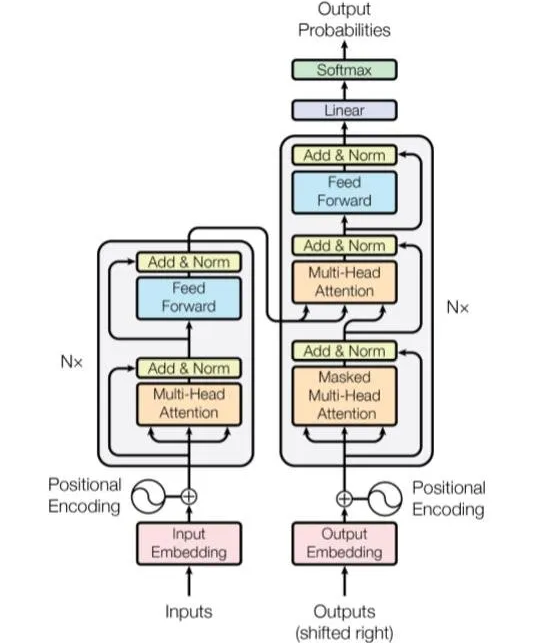
\includegraphics[width=.4\textwidth]{images/transformers_architecture.png}
		\caption{Arquitectura general de un modelo Transformer \parencite{vaswani2017attention}.}
		\label{fig:arquitectura}
	\end{figure}
	
	\item \textbf{Mecanismo de Auto-Atención y Multi-head Attention}:
	
	El componente clave en un Transformer es el mecanismo de auto-atención, que permite al modelo evaluar la importancia de cada palabra en relación con todas las demás palabras dentro de una secuencia.
	
	Para lograr esto, cada palabra en la secuencia se transforma en tres representaciones diferentes: \textbf{Q} (Query), \textbf{K} (Key) y \textbf{V} (Value). La matriz de \textbf{Q} representa la palabra que realiza la consulta, la matriz de \textbf{K} contiene las palabras a comparar y la matriz de \textbf{V} contiene los valores que se combinan según la importancia determinada. La puntuación de atención se obtiene mediante el producto escalar entre \textbf{Q} y \textbf{K}, que luego se normaliza con una función softmax para asignar pesos a \textbf{V}, generando así la representación contextual de cada palabra.
	
	El modelo de \textbf{multi-head attention} permite que el Transformer procese diferentes aspectos del contexto de manera simultánea, representando diversas interpretaciones de las relaciones entre las palabras. Cada cabeza de atención se enfoca en diferentes partes del texto, lo que enriquece la comprensión del modelo sobre los matices semánticos y sintácticos de las palabras \parencite{chopra2013natural}.
	
	La Figura~\ref{fig:atencion} ilustra cómo, a través del mecanismo de auto-atención, el modelo es capaz de identificar y ponderar las relaciones entre distintas palabras de una misma frase, generando así una representación contextual enriquecida de cada token.
	
	\begin{figure}[H]
		\centering
		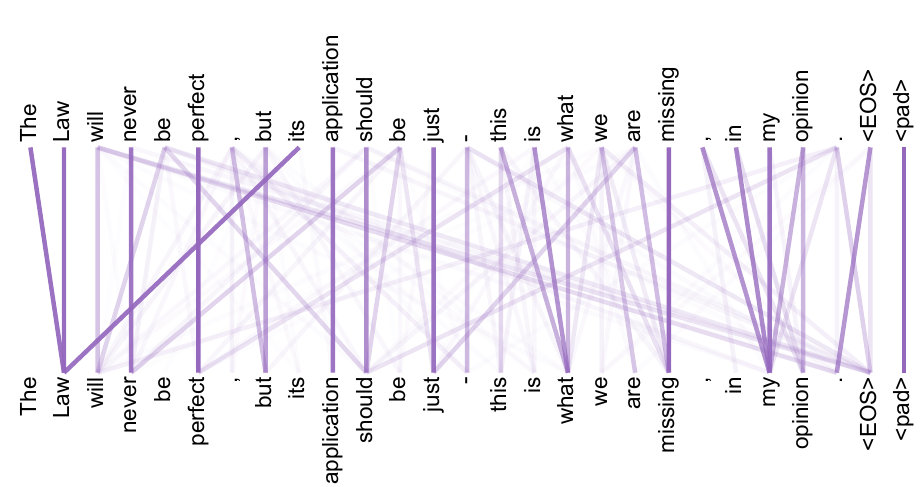
\includegraphics[width=.7\textwidth]{images/clave_valor_atencion.png}
		\caption{Representación del mecanismo de auto-atención, donde se visualiza cómo se establecen relaciones entre palabras de una frase \parencite{vaswani2017attention}.}
		\label{fig:atencion}
	\end{figure}
	
	\item \textbf{Codificación y Decodificación}:
	
	En un Transformer, el proceso se divide en dos fases: codificación y decodificación. El codificador toma la secuencia de entrada y la convierte en una representación interna (vectorial), mientras que el decodificador utiliza esta representación para generar la salida deseada \parencite{vaswani2017attention}.
	
	
\end{itemize}




\subsubsection{Pre-entrenamiento, Fine-Tuning y Destilación de Conocimiento}  
El pre-entrenamiento permite a los LLMs aprender patrones lingüísticos a partir de grandes corpus de texto no etiquetados. Técnicas como Masked Language Modeling (MLM) en BERT y Causal Language Modeling (CLM) en GPT ayudan a capturar la estructura del lenguaje. Posteriormente, el ajuste fino adapta el modelo a tareas específicas mediante conjuntos de datos más pequeños y etiquetados, optimizando su desempeño en aplicaciones concretas \parencite{ren2024learning}.

La destilación de conocimiento es un enfoque para transferir conocimiento de un modelo grande (profesor) a uno más pequeño (estudiante), manteniendo un rendimiento competitivo con menor costo computacional \parencite{sreenivasllm}.


\subsubsection{Generación Aumentada por Recuperación}

El enfoque de \textbf{Generación Aumentada por Recuperación} (Retrieval-Augmented Generation, RAG) representa una técnica híbrida que mejora la capacidad de los modelos de lenguaje para generar texto relevante y fundamentado. Combina un sistema de recuperación de información con un modelo generativo, permitiendo que las respuestas producidas estén respaldadas por datos externos en lugar de depender únicamente del conocimiento almacenado durante el entrenamiento del modelo.

El funcionamiento de un sistema RAG (representado en la Figura \ref{fig:rag_diagrama})puede dividirse en dos etapas principales:

\begin{enumerate}
	\item \textbf{Recuperación}: Ante una consulta, el sistema busca fragmentos de texto relevantes en una base de datos externa. Esta base suele estar implementada como un almacenamiento vectorial, donde los documentos han sido codificados previamente en vectores densos de alta dimensión mediante modelos de embeddings. La similitud semántica entre la consulta y los documentos se calcula utilizando métricas como la distancia coseno.
	
	\item \textbf{Generación}: La información recuperada se proporciona como contexto al modelo generativo (por ejemplo, un Transformer), que genera una respuesta coherente y contextualizada en función tanto de la consulta como del contenido obtenido.
\end{enumerate}

Este enfoque es especialmente útil en tareas que requieren información específica o actualizada, ya que permite complementar el conocimiento estático del modelo con datos en tiempo real. Para que esta recuperación sea eficiente, incluso en bases de datos con millones de vectores, se emplean técnicas como Product Quantization, Hierarchical Navigable Small Worlds (HNSW) o índices aproximados de vecinos más cercanos (ANN) \parencite{lewis2020retrieval}.

\begin{figure}[H]
	\centering
	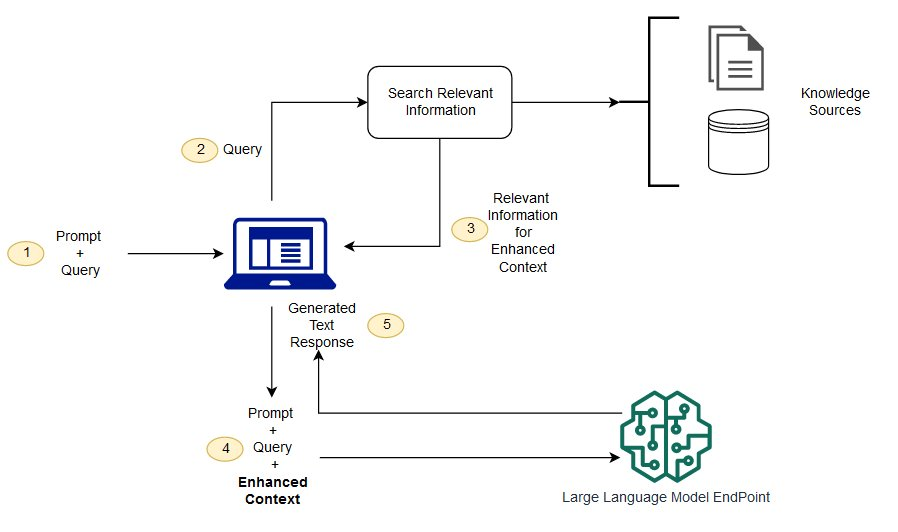
\includegraphics[width=\textwidth]{images/rag_aws.jpg}
	\caption{Funcionamiento general del sistema RAG \parencite{awsRAG}.}
	\label{fig:rag_diagrama}
\end{figure}


\end{document}